\documentclass[aspectratio=169,10pt]{beamer}

\usepackage[utf8]{inputenc}
\usepackage[T1]{fontenc}
\usepackage[spanish,es-nodecimaldot]{babel}
\usepackage{amsmath}
\usepackage{booktabs}
\usepackage{tikz}
\usepackage{graphicx}
\usetikzlibrary{arrows.meta}
\useoutertheme[subsection=false,footline=empty]{miniframes}

\setbeamertemplate{navigation symbols}{}
\setbeamertemplate{frametitle}{%
  \vspace{.14cm}\begin{center}\normalfont\Large\insertframetitle\end{center}\vspace{.08cm}}
\setbeamercolor{normal text}{fg=black,bg=white}
\setbeamercolor{frametitle}{fg=black,bg=white}
\setbeamercolor{itemize item}{fg=black}
\setbeamercolor{section in head/foot}{fg=black,bg=white}
\setbeamercolor{mini frame}{fg=black,bg=white}
\setbeamercolor{upper separation line head}{bg=white}
\setbeamercolor{middle separation line head}{bg=white}
\setbeamercolor{lower separation line head}{bg=white}
\setbeamertemplate{itemize item}{\raise0.15ex\hbox{\large$\bullet$}}
\setbeamertemplate{footline}{}
\setbeamersize{text margin left=1.0cm,text margin right=1.0cm}
\renewcommand{\familydefault}{\sfdefault}

\definecolor{accent}{HTML}{167D8D}
\definecolor{accentlight}{HTML}{E5F1F3}
\newcommand{\metric}[2]{\textbf{#1}\quad #2}
\newcommand{\results}[3]{%
  \begin{tabular*}{\textwidth}{@{\extracolsep{\fill}}lll@{}}#1 & #2 & #3\end{tabular*}}

\begin{document}

% 1. Portada y resultados
\section{Portada}
\begin{frame}
  \vspace{.35cm}
  \begin{center}
    {\LARGE Predicción de la dificultad de pago}\\[.22cm]
    {\normalsize Inteligencia Artificial Explicable --- Unidad 2, Fase II}\\[.35cm]
    {\small Damián Benasco Sánchez \quad Germán Sánchez Carmona \quad Jorge Enrique Vega Ortiz}\\[.3cm]
    {\small 25.000 registros $\cdot$ 15 predictores $\cdot$ 21,21\% de clase positiva}\\[.25cm]

    {\large Validación cruzada anidada: cinco particiones externas}\\[.15cm]
    \renewcommand{\arraystretch}{1.45}
    \begin{tabular}{@{}lr@{}}
      \toprule
      Modelo & ROC-AUC medio \\
      \midrule
      CART & 0,7372 \\
      Regresión logística & 0,7515 \\
      \textbf{EBM} & \textbf{0,7755} \\
      \bottomrule
    \end{tabular}\\[.42cm]
    \textbf{Elegimos EBM: mayor discriminación y quince funciones inspeccionables.}
  \end{center}
\end{frame}

% 2. Árbol CART
\section{CART}
\begin{frame}{Árbol de decisión (CART)}
  \begin{center}
    {\small Partición 1: $P(1)$ en las hojas; resaltadas si $P(1)\geq 0{,}25$.}\\[.05cm]
    \begin{tikzpicture}[
      split/.style={align=center,text width=2.1cm,font=\small,inner sep=2pt},
      root/.style={split,text width=2.35cm},
      leaf/.style={align=center,text width=1.0cm,font=\small,inner sep=3pt},
      positive/.style={leaf,fill=accentlight,draw=accent,rounded corners=2pt},
      edge/.style={-{Stealth[length=1.7mm]},draw=black,line width=.55pt},
      branch/.style={font=\footnotesize,fill=white,inner sep=1pt}
    ]
      \node[root] (r) at (6.1,0) {Estado reciente\\$\leq 0{,}5$?};
      \node[split] (r0) at (3.0,-1.12) {Pago/factura (6m)\\$\leq 0{,}105$?};
      \node[split] (r1) at (9.2,-1.12) {Pago/factura (6m)\\$\leq 0{,}105$?};
      \node[split] (a) at (1.45,-2.28) {Meses sin pago\\$\leq 3{,}5$?};
      \node[split] (b) at (4.55,-2.28) {Meses sin pago\\$\leq 2{,}5$?};
      \node[split] (c) at (7.65,-2.28) {Meses sin pago\\$\leq 2{,}5$?};
      \node[split] (d) at (10.75,-2.28) {Meses sin pago\\$\leq 2{,}5$?};
      \draw[edge] (r) -- node[branch,above left]{sí} (r0);
      \draw[edge] (r) -- node[branch,above right]{no} (r1);
      \draw[edge] (r0) -- node[branch,above left]{sí} (a);
      \draw[edge] (r0) -- node[branch,above right]{no} (b);
      \draw[edge] (r1) -- node[branch,above left]{sí} (c);
      \draw[edge] (r1) -- node[branch,above right]{no} (d);
      \node[leaf] (l1) at (.7,-3.48) {0,192};
      \node[positive] (l2) at (2.2,-3.48) {0,406};
      \node[leaf] (l3) at (3.8,-3.48) {0,072};
      \node[leaf] (l4) at (5.3,-3.48) {0,121};
      \node[positive] (l5) at (6.9,-3.48) {0,465};
      \node[positive] (l6) at (8.4,-3.48) {0,693};
      \node[leaf] (l7) at (10.0,-3.48) {0,193};
      \node[positive] (l8) at (11.5,-3.48) {0,283};
      \draw[edge] (a) -- node[branch,above left]{sí} (l1.north);
      \draw[edge] (a) -- node[branch,above right]{no} (l2.north);
      \draw[edge] (b) -- node[branch,above left]{sí} (l3.north);
      \draw[edge] (b) -- node[branch,above right]{no} (l4.north);
      \draw[edge] (c) -- node[branch,above left]{sí} (l5.north);
      \draw[edge] (c) -- node[branch,above right]{no} (l6.north);
      \draw[edge] (d) -- node[branch,above left]{sí} (l7.north);
      \draw[edge] (d) -- node[branch,above right]{no} (l8.north);
    \end{tikzpicture}
  \end{center}
  \vspace{-.08cm}
  \begin{center}
    \results{\metric{ROC-AUC}{0,7372 $\pm$ 0,0044}}{\metric{Exac. equilibrada}{67,3\%}}{\metric{Sensibilidad}{48,9\%}}\\[.08cm]
    {\footnotesize Validación externa en cinco particiones; métricas de clasificación con umbral 0,25.}
  \end{center}
\end{frame}

% 3. Regresión logística
\section{Regresión logística}
\begin{frame}{Regresión logística: variables más relevantes}
  \begin{center}\small
    $\operatorname{logit}(p)=\beta_0+\sum_j\beta_j z_j$
    \quad Coeficientes de la partición 1: L1, $C=0{,}1$.
  \end{center}
  \vspace{-.1cm}
  \begin{columns}[c,onlytextwidth]
    \begin{column}{.67\textwidth}
      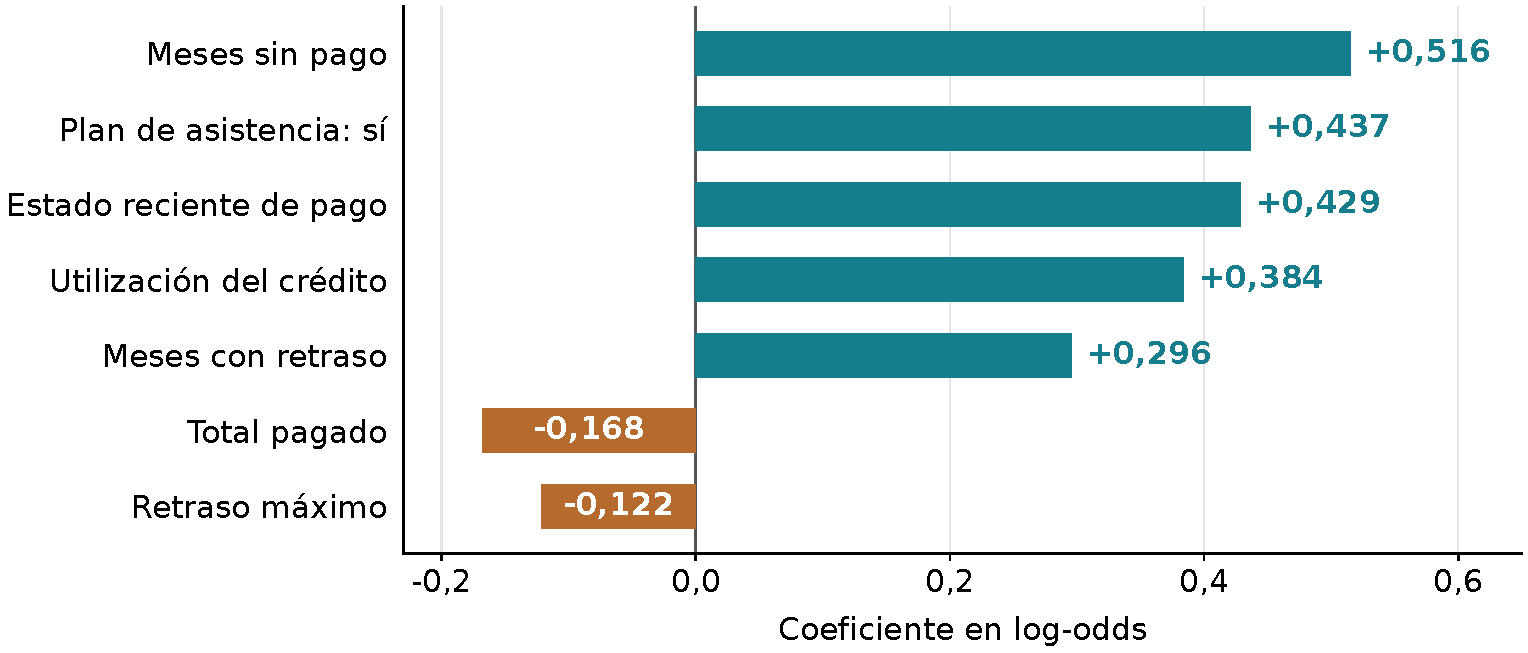
\includegraphics[width=\linewidth,height=3.85cm,keepaspectratio]{logistic_coefficients.pdf}\\[-.02cm]
      {\scriptsize Numéricas por una desviación típica; plan: sí frente a no.}
    \end{column}
    \begin{column}{.30\textwidth}
      \footnotesize
      {\color{accent}\bfseries Variables más relevantes}\\[.12cm]
      \textbf{Meses sin pago, estado reciente y utilización:} asociación positiva con la dificultad.\\[.12cm]
      \textbf{Plan de asistencia:} también tiene coeficiente positivo.\\[.12cm]
      \textbf{Total pagado:} asociación negativa, manteniendo el resto constante.
    \end{column}
  \end{columns}
  \begin{center}\small
    \results{\metric{ROC-AUC}{0,7515 $\pm$ 0,0075}}{\metric{Exac. equilibrada}{68,1\%}}{\metric{Sensibilidad}{59,6\%}}\\[.06cm]
    {\scriptsize Medias externas de cinco particiones; umbrales internos 0,20 o 0,25. Asociaciones, no causas.}
  \end{center}
\end{frame}

% 4. EBM
\section{EBM}
\begin{frame}{EBM: una relación no lineal y una decisión local}
  \begin{center}\small
    $\operatorname{logit}(p)=\beta_0+\sum_{j=1}^{15}f_j(x_j)$
    \quad Quince funciones, sin interacciones.
  \end{center}
  \vspace{-.1cm}
  \begin{columns}[c,onlytextwidth]
    \begin{column}{.65\textwidth}
      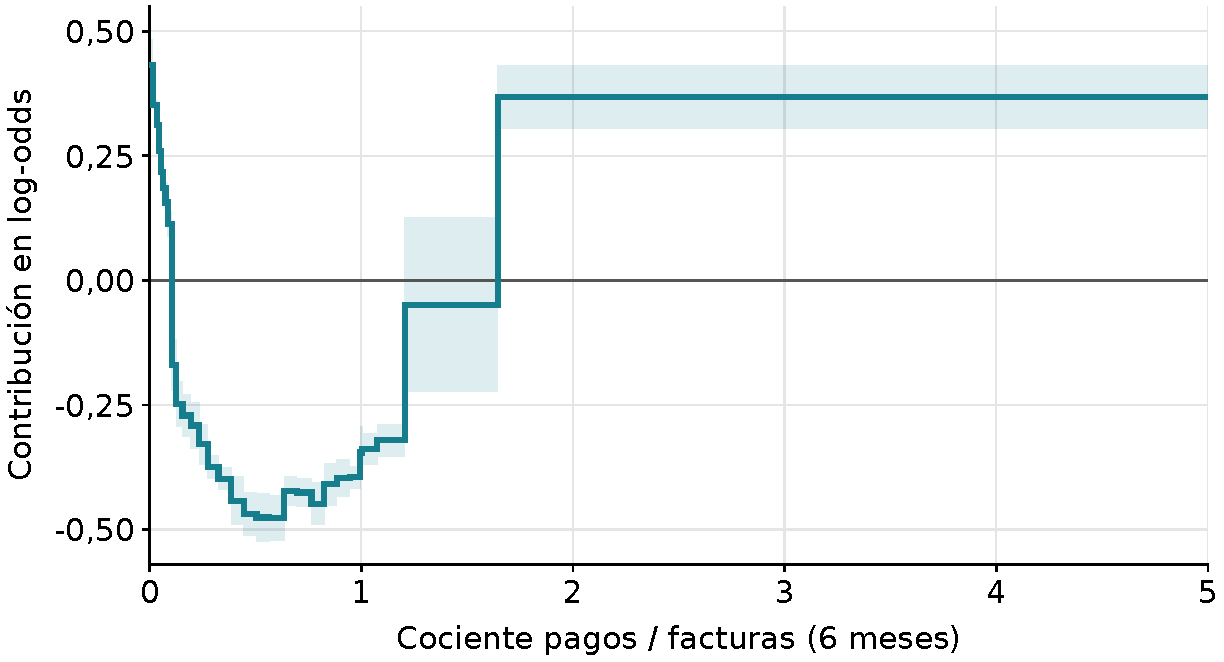
\includegraphics[width=\linewidth,height=3.85cm,keepaspectratio]{ebm_payment_to_bill_ratio.pdf}\\[-.05cm]
      {\scriptsize Partición 1. Bandas: variabilidad entre réplicas de bagging.}
    \end{column}
    \begin{column}{.32\textwidth}
      \small
      {\color{accent}\bfseries Relación no monótona}\\[.12cm]
      Positiva en los extremos; negativa en valores intermedios.\\[.22cm]
      {\color{accent}\bfseries Caso 3: clase real 0}\\[.12cm]
      {\footnotesize El cociente aporta $+0{,}352$ log-odds.}\\[.08cm]
      $P(1)=21{,}10\%$\\
      Umbral: $20\%$\\
      $\Rightarrow$ \textbf{falso positivo}.\\[.12cm]
      {\footnotesize Árbol y logística aciertan. La ventaja media no garantiza acertar cada caso.}
    \end{column}
  \end{columns}
  \begin{center}\small
    \results{\metric{ROC-AUC}{0,7755 $\pm$ 0,0077}}{\metric{Exac. equilibrada}{70,0\%}}{\metric{Sensibilidad}{64,1\%}}\\[.06cm]
    {\scriptsize Cinco particiones externas; umbrales 0,20 o 0,25. Más detección, más falsas alertas.}
  \end{center}
\end{frame}

\end{document}
